\section{The indirect-gap window}\label{sec:13.1}

A dark-matter particle of \SI{0.35}{MeV} can deposit up to $\frac12\mchi v_{\mathrm{max}}^2 = \SI{1.23}{eV}$, more than the \SI{1.17}{eV} gap of silicon, but only at the momentum transfer $q = \mchi v_{\mathrm{max}} = \SI{0.93}{keV}$. This momentum transfer is less than half of the \SI{1.94}{keV} that separates the valence-band maximum from the conduction valleys, and at $q = \SI{0.93}{keV}$ the cheapest electron--hole pair along the valley axis costs about \SI{1.9}{eV} (\cref{fig:3-si-bands}). Without a phonon the particle cannot create a pair. With a phonon of about \SI{15}{meV} that takes up the remaining \SI{1.0}{keV} of the valley momentum, it can. The phonon-assisted process of \cref{sec:9.1} is then the only way for dark matter scattering on electrons to create an electron--hole pair, in a window of masses that runs from the lightest mass that creates a pair with a phonon, $m_{\mathrm{min}}^{\mathrm{PA}}$, to the lightest mass that creates a pair without a phonon, $m_{\mathrm{min}}^{\mathrm{ZP}}$.

\subsection{The zero-phonon threshold mass}

The largest momentum transfer of a particle of mass $\mchi$ is $2\mchi v_{\mathrm{max}}$, and it reaches the valley momentum $k_{\mathrm{c}} = \SI{1.94}{keV}$ of \cref{eq:3.3-kc} only for $\mchi \ge k_{\mathrm{c}}/2v_{\mathrm{max}} = \SI{0.366}{MeV}$; at that mass the particle reaches $k_{\mathrm{c}}$ by backscattering, with no energy to spare. The energy that the particle can deposit at fixed $q$ is $qv_{\mathrm{max}} - q^2/2\mchi$ (\cref{eq:1.3-region}), largest at $q = \mchi v_{\mathrm{max}}$. The two requirements conflict: depositing the gap favors $q \approx \mchi v_{\mathrm{max}}$, while reaching the valley needs $q \approx k_{\mathrm{c}}$, and for light particles $\mchi v_{\mathrm{max}}$ is well below $k_{\mathrm{c}}$.

To locate the zero-phonon threshold, we turn the kinematic condition \cref{eq:3.3-allowed} into a condition on the mass. At fixed $\vect{q}$, a pair of energy $E$ is reachable when $qv_{\mathrm{max}} - q^2/2\mchi \ge E$. For $qv_{\mathrm{max}} > E$ this condition reads
\begin{equation*}
  \mchi \ge \frac{q^2}{2\,(qv_{\mathrm{max}} - E)} .
\end{equation*}
The right-hand side grows with $E$ at fixed $q$, so at each $\vect{q}$ the cheapest pair sets the bound, and the energy of that pair is the minimum pair energy $E_{\mathrm{min}}(\vect{q})$ of \cref{eq:3.3-Emin}. Minimizing then over $\vect{q}$, and writing out the minimum over the hole's crystal momentum $\vect{k}$ that $E_{\mathrm{min}}$ contains, gives the zero-phonon threshold mass
\begin{equation}
  m_{\mathrm{min}}^{\mathrm{ZP}} = \min_{\vect{q}}\frac{q^2}{2\,[qv_{\mathrm{max}} - E_{\mathrm{min}}(\vect{q})]}
  = \min_{\vect{q},\,\vect{k},\,v,\,c}\frac{q^2}{2\,[qv_{\mathrm{max}} - \varepsilon_{c,\vect{k}+\vect{q}} + \varepsilon_{v\vect{k}}]} ,
  \label{eq:13.1-mZP}
\end{equation}
with the minimum over the region where the denominator is positive. The second form is one minimization over six continuous variables, three for $\vect{q}$ and three for $\vect{k}$, and it shows that two common simplifications, fixing the hole at the valence-band maximum and restricting $\vect{q}$ to a few directions, can only raise the result.

Near a valley the minimization can be done by hand. Along the axis of a silicon valley, the pair energy is the parabola \cref{eq:3.3-Eminpar}, $E_{\mathrm{min}} \simeq \Eg + (q - k_{\mathrm{c}})^2/2M_{\mathrm{eh}}$, where $M_{\mathrm{eh}} = m^*_\parallel + m_{\mathrm{hh}}$ is the mass with which the pair as a whole recoils, equal to the sum of the longitudinal electron mass and the heavy-hole mass in the same direction. With $m^*_\parallel = 0.916\,m_e$ and $m_{\mathrm{hh}} = 0.277\,m_e$ along [100] (\cref{tab:3-materials}), $M_{\mathrm{eh}} = 1.19\,m_e$. Inserted in \cref{eq:13.1-mZP}, the parabola gives $m_{\mathrm{min}}^{\mathrm{ZP}} = \SI{0.425}{MeV}$ at $q = \SI{1.46}{keV}$. At that point the particle falls \SI{0.48}{keV} short of the valley, and the pair absorbs the shortfall as kinetic energy, $(\SI{0.48}{keV})^2/2M_{\mathrm{eh}} = \SI{0.19}{eV}$, for a total pair energy of \SI{1.36}{eV}. Lighter particles would have to transfer still less momentum, and the kinetic energy of the pair grows quadratically with the shortfall while the energy available grows only linearly with $\mchi$. The first-principles bands of \cref{fig:3-si-bands}, used along the same axis, give \SI{0.420}{MeV} at $q = \SI{1.43}{keV}$.

The pair need not move along the valley axis, and the hole need not sit at the valence-band maximum; the heavy-hole surfaces of silicon are strongly warped (\cref{eq:3.3-holes}), and a hole that moves into a flat direction lowers the kinetic energy of the pair. The full minimization \cref{eq:13.1-mZP} therefore gives a threshold mass below \SI{0.42}{MeV}, off the axis. \Cref{sec:13.9} gives its value and explains why the first zero-phonon states reached at that threshold are weakly coupled. Binding the pair into an exciton changes the threshold mass only slightly. The $1s$ exciton lies $E_x^b = \SI{14.7}{meV}$ below the free pair (\cref{sec:4.9}). Since $\partial\mchi/\partial E = \mchi/(qv_{\mathrm{max}} - E)$ at fixed $q$, the exciton lowers the threshold mass by $\mchi E_x^b/(qv_{\mathrm{max}} - E) = \SI{0.0025}{MeV}$ at the parabolic optimum, about \SI{0.6}{\percent}.

\subsection{The phonon-assisted onset}

A phonon changes the bookkeeping of crystal momentum. The dark matter transfers $\vect{q}$; the electron ends at $\vect{k}_e$ in a conduction band, the hole at $\vect{k}_h$ in a valence band, and a phonon of branch $\nu$ and wavevector $\vect{Q}$ is emitted. Conservation of crystal momentum fixes $\vect{Q} = \vect{k}_e - \vect{k}_h - \vect{q}$ up to a reciprocal-lattice vector, and the energy deposited is $\varepsilon_{c\vect{k}_e} - \varepsilon_{v\vect{k}_h} + \omega_{\vect{Q}\nu}$. The phonon takes whatever crystal momentum the pair needs, and since no phonon of silicon has more than \SI{64}{meV} (\cref{sec:5.2}), that momentum costs at most a few percent of the gap. The cheapest final state puts the electron at the bottom of a valley and the hole at the valence-band maximum. At momentum transfer $\vect{q}$ it costs
\begin{equation}
  E_{\mathrm{min}}^{\mathrm{PA}}(\vect{q}) = \Eg + \min_\nu\,\omega_{\vect{k}_{\mathrm{c}} - \vect{q},\,\nu} ,
  \label{eq:13.1-EPA}
\end{equation}
with $\vect{k}_{\mathrm{c}}$ the valley that makes the phonon cheapest, chosen among the six valleys and their images under reciprocal-lattice vectors. Compared to the zero-phonon edge, the phonon-assisted threshold hardly depends on $\vect{q}$. It falls to $\Eg$ only at $\vect{q} = \vect{k}_{\mathrm{c}}$, where the acoustic phonon needed has zero energy, and it never rises above $\Eg + \SI{64}{meV}$. Moving the electron and the hole off the band extrema could lower the phonon energy but adds kinetic energy to the pair. With the dispersion of \cref{sec:5.2}, the best trade between phonon energy and kinetic energy lowers the threshold by less than \SI{0.02}{meV}, an amount we neglect.

\Cref{eq:13.1-EPA} assumes that the phonon is emitted. At temperature $T$ the pair can also be created by absorbing a phonon. Absorption costs $\Eg - \omega_{\vect{Q}\nu}$ but comes with the occupation $n_{\mathrm{B}}(\omega_{\vect{Q}\nu})$ in place of $n_{\mathrm{B}} + 1$ (\cref{sec:5.3}), and $\Eg$ itself shifts with $T$ (\cref{sec:13.7}). For the transverse acoustic phonon of about \SI{15}{meV} that sets the onset below, $n_{\mathrm{B}}$ is 0.12 at \SI{77}{K}, $2\times10^{-19}$ at \SI{4}{K} and $3\times10^{-75}$ at \SI{1}{K}. The absorption sideband, which would open at \SI{0.329}{MeV}, is absent in a detector at millikelvin temperatures. At those temperatures only emission counts, and $\Eg$ is the gap extrapolated to zero temperature.

The onset mass follows from \cref{eq:13.1-EPA} as $m_{\mathrm{min}}^{\mathrm{ZP}}$ followed from $E_{\mathrm{min}}$:
\begin{equation}
  m_{\mathrm{min}}^{\mathrm{PA}} = \min_{\vect{q}}\frac{q^2}{2\,[qv_{\mathrm{max}} - E_{\mathrm{min}}^{\mathrm{PA}}(\vect{q})]} .
  \label{eq:13.1-mPAdef}
\end{equation}
For a threshold $E$ independent of $q$, the minimum sits at $q = 2E/v_{\mathrm{max}}$ and equals the floor $2E/v_{\mathrm{max}}^2$ of \cref{eq:1.3-mmin}. Here $E$ varies with $q$, but slowly. Write $E(q)$ for $E_{\mathrm{min}}^{\mathrm{PA}}$ along a line of $\vect{q}$ and $E' = \dd E/\dd q$. Setting the derivative of $q^2/[2(qv_{\mathrm{max}} - E)]$ to zero gives $qv_{\mathrm{max}} - 2E + qE' = 0$. The optimum is therefore $q^* = 2E/(v_{\mathrm{max}} + E')$, and inserting $q^*$ back into \cref{eq:13.1-mPAdef} gives
\begin{equation}
  m_{\mathrm{min}}^{\mathrm{PA}} = \frac{2\,[\Eg + \omega_\nu(\vect{Q}^*)]}{v_{\mathrm{max}}^2 - u_\nu^2} ,
  \qquad \vect{Q}^* = \vect{k}_{\mathrm{c}} - \vect{q}^* ,\quad q^* \simeq \frac{2\,[\Eg + \omega_\nu(\vect{Q}^*)]}{v_{\mathrm{max}}} ,
  \label{eq:13.1-mPA}
\end{equation}
where $u_\nu = |E'|$ is the group velocity of the phonon along $\vect{q}$ at $\vect{Q}^*$ and the branch $\nu$ is the one that gives the smallest result. The slope of the dispersion enters only squared, because $q^*$ is a stationary point: moving $q$ slightly changes the phonon energy to first order but the mass only to second. Phonon group velocities are a few km/s, below the speeds of sound, against $v_{\mathrm{max}} = \SI{794.5}{km.s^{-1}}$, and $u_\nu^2/v_{\mathrm{max}}^2 \sim 10^{-5}$. To that accuracy the onset is the kinematic floor with the gap raised by the energy of one phonon, at the wavevector $\vect{Q}^*$ that the dark matter leaves for the phonon. \Cref{eq:13.1-mPA} is implicit, since $\vect{Q}^*$ depends on $q^*$, but one or two iterations starting from $\omega = 0$ settle the value of $q^*$.

\begin{keyresult}[Window kinematics]
In an indirect-gap crystal at zero temperature, scattering dark matter creates an electron--hole pair only above the phonon-assisted onset $m_{\mathrm{min}}^{\mathrm{PA}}$ of \cref{eq:13.1-mPA}, and without a phonon only above the zero-phonon threshold $m_{\mathrm{min}}^{\mathrm{ZP}}$ of \cref{eq:13.1-mZP}. For
\begin{equation*}
  m_{\mathrm{min}}^{\mathrm{PA}} \le \mchi < m_{\mathrm{min}}^{\mathrm{ZP}} ,
\end{equation*}
the phonon-assisted process is the only electron-recoil channel. Bound pairs lower both edges of the window by replacing $\Eg$ with $\Eg - E_x^b$ in the corresponding threshold.
\end{keyresult}

The onset is set by the branch of lowest energy at $\vect{Q}^*$, whatever its coupling strength. In silicon the transverse acoustic (TA) branch is the lowest everywhere away from the zone center, and \cref{we:13-onset} finds $\omega_{\mathrm{TA}}(\vect{Q}^*) = \SI{14.8}{meV}$ at $|\vect{Q}^*| = 0.46\,(2\pi/a)$, with $\vect{q}^*$ along the valley axis. Tilting $\vect{q}$ away from the axis raises the TA energy at $\vect{Q}^*$, by \SI{0.7}{meV} at a tilt of \SI{0.3}{rad} in a $\{001\}$ plane, so the onset is on the axis. The longitudinal acoustic and transverse optical branches open later, at 0.341 and \SI{0.350}{MeV}. Compared to light, dark matter needs a phonon of shorter wavevector and lower energy. A photon carries no momentum on the scale of the zone, so in optical absorption the phonon must supply all of $\vect{k}_{\mathrm{c}}$, and the TA phonon that sets the optical edge has \SI{18.27}{meV}~\cite{macfarlane1958fine} (\cref{sec:6.5}). A particle at the onset supplies $q^* = \SI{0.90}{keV}$ itself, about half of $k_{\mathrm{c}}$, and leaves the phonon a shorter wavevector on the flat part of the TA branch.

\Cref{fig:13-window} puts the two thresholds side by side. In panel (a) the zero-phonon edge $E_{\mathrm{min}}(\vect{q})$ dips to $\Eg$ only near $k_{\mathrm{c}}$, while the phonon-assisted threshold \cref{eq:13.1-EPA} runs almost flat just above $\Eg$ at every $q$. The parabola of a \SI{0.3}{MeV} particle stays below both thresholds. The parabola of a \SI{0.4}{MeV} particle crosses the phonon-assisted threshold but not, along these directions, the zero-phonon edge; a \SI{0.5}{MeV} particle reaches both thresholds. Panel (b) shows the same comparison as two curves of threshold mass against $q$, and the minima of the two curves are \cref{eq:13.1-mZP,eq:13.1-mPAdef}: the phonon-assisted curve has a broad minimum near \SI{0.9}{keV}, the zero-phonon curve a narrow one near \SI{1.4}{keV}.

\begin{figure}[tbp]
  \centering
  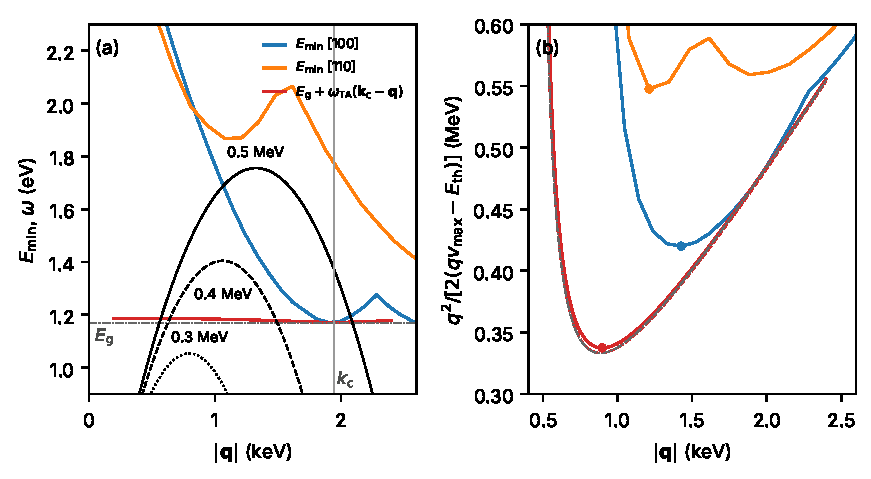
\includegraphics[width=\linewidth]{figures/ch13/fig13_1.pdf}
  \caption{Kinematics of the indirect-gap window of silicon. (a)~Minimum pair energy $E_{\mathrm{min}}(\vect{q})$ (\cref{eq:3.3-Emin}) for $\vect{q}$ along [100] and [110], and the phonon-assisted threshold $\Eg + \omega_{\mathrm{TA}}(\vect{k}_{\mathrm{c}} - \vect{q})$ (\cref{eq:13.1-EPA}) for $\vect{q}$ along [100], with the electron at the valley minimum $\vect{k}_{\mathrm{c}} = 0.85\,(2\pi/a)(1,0,0)$ and the hole at the valence-band maximum. Black: the largest energy deposited, $qv_{\mathrm{max}} - q^2/2\mchi$, for $\mchi = 0.3$ (dotted), 0.4 (dashed) and \SI{0.5}{MeV} (solid), with $v_{\mathrm{max}} = 2.650\times10^{-3}$. Dash-dotted: $\Eg = \SI{1.17}{eV}$. (b)~The lightest mass that reaches each threshold at momentum transfer $q$, $q^2/[2(qv_{\mathrm{max}} - E_{\mathrm{th}})]$; dots mark the minima over $q$. Red solid: phonon-assisted, free pair, minimum \SI{0.3374}{MeV} at $q = \SI{0.90}{keV}$; red dashed: bound pair, $\Eg$ lowered by $E_x^b = \SI{14.7}{meV}$, minimum \SI{0.3332}{MeV}; grey dash-dotted: the floor $2\Eg/v_{\mathrm{max}}^2$ at fixed threshold $\Eg$. Blue and orange: zero-phonon, with minima \SI{0.420}{MeV} along [100] and \SI{0.548}{MeV} along [110]; these are upper values for the zero-phonon threshold, since the joint minimum over all directions of $\vect{q}$ and all hole momenta lies lower. The [111] direction, whose $E_{\mathrm{min}}$ stays above \SI{2.13}{eV}, is off scale (minimum \SI{0.615}{MeV}). Bands: PBE calculation of \cref{fig:3-si-bands} at $a = \SI{5.431}{\angstrom}$ on a grid of $48^3$ crystal momenta, without spin--orbit coupling, with the conduction bands shifted up by \SI{0.613}{eV} so that the indirect gap equals the measured \SI{1.17}{eV}. Phonons: PBE force constants of \cref{sec:5.2} at the same lattice constant. The TA branch of these force constants is \SI{8}{\percent} below the neutron data at X, and scaling it up to the data raises the phonon-assisted minimum to \SI{0.3378}{MeV}.}
  \label{fig:13-window}
\end{figure}

\begin{workedexample}{The phonon-assisted onset of silicon}\label{we:13-onset}
We evaluate \cref{eq:13.1-mPA} with the measured gap extrapolated to zero temperature, $\Eg = \SI{1.17}{eV}$, the valley at $k_{\mathrm{c}} = 0.85\,(2\pi/a) = \SI{1940}{eV}$ (\cref{we:3-kc}), $v_{\mathrm{max}}^2 = 7.023\times10^{-6}$, and the TA branch of the force constants of \cref{sec:5.2}, with $\vect{q}$ along the valley axis.

\emph{First pass, no phonon energy.} $q^* = 2\Eg/v_{\mathrm{max}} = \SI{883}{eV}$, which leaves the phonon $Q^* = k_{\mathrm{c}} - q^* = \SI{1057}{eV} = 0.463\,(2\pi/a)$. The TA energy there is \SI{14.87}{meV}.

\emph{Second pass.} With $E = \Eg + \omega_{\mathrm{TA}}(\vect{Q}^*) = \SI{1.1849}{eV}$, $q^* = 2E/v_{\mathrm{max}} = \SI{894}{eV}$ and $Q^* = 0.458\,(2\pi/a) = \SI{0.53}{\angstrom^{-1}}$, where $\omega_{\mathrm{TA}}(\vect{Q}^*) = \SI{14.79}{meV}$. A third pass changes nothing at this precision. The slope of the TA branch at $Q^*$ is $u_{\mathrm{TA}} = \SI{2.1}{km.s^{-1}}$, and $u_{\mathrm{TA}}^2/v_{\mathrm{max}}^2 = 7\times10^{-6}$ is negligible. The onset is
\begin{equation*}
  m_{\mathrm{min}}^{\mathrm{PA}} = \frac{2\times(\SI{1.17}{eV} + \SI{0.01479}{eV})}{7.023\times10^{-6}} = \SI{0.3374}{MeV} ,
\end{equation*}
\SI{1.3}{\percent} above the floor $2\Eg/v_{\mathrm{max}}^2 = \SI{0.3332}{MeV}$. The direct minimization of \cref{eq:13.1-mPAdef} on a grid of $q$ gives the same value, at $q = \SI{0.90}{keV}$.

\emph{Sensitivity.} An error $\delta\omega$ in the phonon energy moves the onset by $2\,\delta\omega/v_{\mathrm{max}}^2 = \SI{2.8e-4}{MeV}$ per meV. The TA branch of this calculation is \SI{8}{\percent} soft at X; scaling the whole branch up to the neutron value there gives $\omega_{\mathrm{TA}}(\vect{Q}^*) = \SI{16.1}{meV}$ and an onset of \SI{0.3378}{MeV}. Had the phonon to supply all of $\vect{k}_{\mathrm{c}}$, as for light, the \SI{18.27}{meV} of the optical edge would put the onset at \SI{0.3384}{MeV}.

\emph{Bound pair.} The $1s$ exciton replaces $\Eg$ by $\Eg - E_x^b = \SI{1.1553}{eV}$. The same passes give $q^* = 2E/v_{\mathrm{max}} = \SI{0.883}{keV}$, where $\omega_{\mathrm{TA}}(\vect{Q}^*) = \SI{14.87}{meV}$, and the onset becomes $2\times\SI{1.1702}{eV}/v_{\mathrm{max}}^2 = \SI{0.3332}{MeV}$; the direct minimization puts the optimum at \SI{0.885}{keV} with the same onset. The phonon energy and the binding energy nearly cancel, and the bound-pair onset falls on the floor $2\Eg/v_{\mathrm{max}}^2$ that a crystal with a direct gap of \SI{1.17}{eV} would have. The strength of this phonon replica of the $1s$ exciton, compared with the free-pair continuum above it, is a question for \cref{sec:13.8}.
\end{workedexample}

\subsection{Germanium and a direct-gap crystal}

Germanium has its valleys at the L points, at $|\vect{k}_{\mathrm{c}}| = |\mathrm{\Gamma}\mathrm{L}| = \SI{1.90}{keV}$, almost the momentum of the silicon valleys, but a gap of only \SI{0.744}{eV} (\cref{sec:3.3}). Its floor $2\Eg/v_{\mathrm{max}}^2$ is \SI{0.212}{MeV}, at $q = \SI{0.56}{keV}$, and the phonon must supply the remaining \SI{1.34}{keV}, about 0.7 of the way from $\mathrm{\Gamma}$ to L. Along that line the transverse acoustic branch of germanium rises monotonically to \SI{1.9}{THz}, \SI{7.9}{meV}, at L~\cites{nilsson1971phonon}[Table~IV]{haxhijaj2026lattice}, so $\omega_{\mathrm{TA}}(\vect{Q}^*) \le \SI{7.9}{meV}$, and \cref{eq:13.1-mPA} places the phonon-assisted onset between 0.2119 and \SI{0.2141}{MeV}. The bracket needs no band structure and no computed phonon, only the gap, the position of L and the measured TA branch.

The zero-phonon threshold of germanium is harder to pin down. \Cref{we:3-mmin} bracketed it between 0.212 and \SI{0.420}{MeV}. On the L axis, with the parabola of \cref{eq:3.3-Eminpar} and $M_{\mathrm{eh}} = m^*_\parallel + m_{\mathrm{hh}} = (1.59 + 0.469)\,m_e = 2.06\,m_e$ along [111] (\cref{tab:3-materials}), \cref{eq:13.1-mZP} gives \SI{0.32}{MeV} at $q = \SI{1.10}{keV}$. The heavy longitudinal mass of the L valleys makes the kinetic energy of the momentum shortfall small, and the zero-phonon edge sits much closer to the onset, in relative terms, than in silicon. The value of \SI{0.32}{MeV} is a guide, not a bound on the zero-phonon edge: the minimum need not lie on the axis, and the heavy hole of germanium is warped and strongly mixed by spin--orbit coupling ($\Delta_{\mathrm{SO}} = \SI{0.296}{eV}$). \Cref{sec:13.9-ge-gaas} states what is known of the edge.

The route through the direct gap at $\mathrm{\Gamma}$ plays no part: as \cref{we:3-mmin} showed, the light pair at the direct gap opens only at a few MeV.

A direct-gap crystal has a window as well. Take GaAs, with both band edges at $\mathrm{\Gamma}$ and a gap of \SI{1.52}{eV}. Its floor is $2\Eg/v_{\mathrm{max}}^2 = \SI{0.433}{MeV}$, and below that mass dark matter scattering creates no pair in GaAs, with or without a phonon. At the masses of the silicon and germanium windows a direct-gap crystal of this gap has no electron-recoil channel. Above the floor, however, energy and momentum conflict again. A pair at rest at $\mathrm{\Gamma}$ costs exactly $\Eg$, but the particle deposits $\Eg$ only near $q^* = 2\Eg/v_{\mathrm{max}} = \SI{1.15}{keV}$, and a zero-phonon pair that carries this momentum has kinetic energy $q^{*2}/2M_{\mathrm{eh}}$. The electron of GaAs is light, $0.067\,m_e$, and with a heavy hole along [100] or [111] the pair mass is $M_{\mathrm{eh}} = 0.42$ or $0.96\,m_e$, and the kinetic energy is 3.1 or \SI{1.3}{eV}, comparable to the gap itself. For a pair of mass $M_{\mathrm{eh}}$ at $\mathrm{\Gamma}$, the condition for the pair to be reachable is $qv_{\mathrm{max}} - q^2/2\mchi - q^2/2M_{\mathrm{eh}} \ge \Eg$. Its left-hand side is largest at $q = \mu v_{\mathrm{max}}$, with $\mu = \mchi M_{\mathrm{eh}}/(\mchi + M_{\mathrm{eh}})$, where it equals $\frac12\mu v_{\mathrm{max}}^2$. Writing $m_{\mathrm{g}} = 2\Eg/v_{\mathrm{max}}^2$ for the floor, the zero-phonon threshold of a direct gap is therefore
\begin{equation}
  m_{\mathrm{min}}^{\mathrm{ZP}} = \frac{m_{\mathrm{g}}M_{\mathrm{eh}}}{M_{\mathrm{eh}} - m_{\mathrm{g}}} \qquad (M_{\mathrm{eh}} > m_{\mathrm{g}}) ,
  \label{eq:13.1-mZPdir}
\end{equation}
and there is none when $M_{\mathrm{eh}} \le m_{\mathrm{g}}$. For GaAs, $m_{\mathrm{g}} = 0.847\,m_e$: in the parabolic approximation, the pair with the [100] heavy hole never opens, and the pair with the [111] heavy hole opens at \SI{3.7}{MeV}. A phonon supplies the momentum, as in silicon: it carries $\vect{Q} \approx -\vect{q}^*$, about half the way to the zone boundary, and leaves the pair at rest. The transverse acoustic branch is the cheapest, and it stays below the \SI{10.5}{meV} that the computed dispersion gives at X (\cref{tab:5-phonons}). The computed \SI{10.5}{meV} is an upper value, since the computed branch lies above the measured one at X, and \cref{eq:13.1-mPA} gives an onset of 0.433 to \SI{0.436}{MeV}. The first zero-phonon states that a particle near this mass can reach are the states of the L valleys, which lie \SI{1.815}{eV} above the valence-band maximum, at $|\mathrm{\Gamma}\mathrm{L}| = \SI{1.90}{keV}$ (\cref{sec:3.3}). Their floor is $2\times\SI{1.815}{eV}/v_{\mathrm{max}}^2 = \SI{0.517}{MeV}$, and depositing \SI{1.815}{eV} at exactly $|\mathrm{\Gamma}\mathrm{L}|$ needs \SI{0.560}{MeV}, so the zero-phonon edge of the L valleys lies between 0.517 and \SI{0.560}{MeV}. GaAs therefore has a phonon-assisted window too, from \SI{0.43}{MeV} to above \SI{0.5}{MeV}, but it begins above the masses at which the silicon window has already closed.

A window thus exists in any crystal whose pairs cannot absorb the momentum $q^* \approx 2\Eg/v_{\mathrm{max}}$ for less than a phonon energy, that is, whenever $|\vect{q}^* - \vect{k}_{\mathrm{c}}|^2/2M_{\mathrm{eh}}$ exceeds the phonon energies at the corresponding $\vect{Q}^*$. For band masses of order $m_e$ and $q^* \sim \SI{1}{keV}$ the kinetic energy of the pair is of order an eV, a hundred times a phonon energy, and the condition is met in silicon, germanium and GaAs alike. In silicon and germanium the indirect gap places the windows low. The two windows start at the floors of their crystals, 0.333 and \SI{0.212}{MeV}, where no direct-gap crystal of comparable gap has any electron recoil. The optical absorption edges of silicon and germanium are phonon-assisted, and they measure the same kind of amplitude in the limit $q \to 0$ (\cref{sec:13.5}).
